\documentclass[unknownkeysallowed,xcolor=table]{beamer}
 
\usepackage[T2A,T1]{fontenc}
\usepackage[utf8]{inputenc}
\usepackage[english,russian]{babel}
\usepackage{listings}
\usepackage{amsmath}
\usepackage{url}
\usepackage{textcomp}
\usepackage{multirow}
\usepackage{tikz}

\setbeamertemplate{navigation symbols}{}

\newcommand{\textapprox}{\raisebox{0.5ex}{\texttildelow}}

\newcommand{\rarr}{$\rightarrow$}
 
\colorlet{mygreen}{green!60!blue}
\colorlet{mymauve}{red!60!blue}
\definecolor{light-gray}{gray}{0.9}

\lstset{
      basicstyle=\ttfamily\small,
      commentstyle=\color{mygreen},
      keywordstyle=\color{blue},
      numberstyle=\tiny\color{blue},
      stringstyle=\color{mymauve},
      numbers=left,
      stepnumber=1,
      columns=fullflexible,
      breaklines=true,
      postbreak=\mbox{\textcolor{red}{\ensuremath{\hookrightarrow}\space}},
      literate={~} {\textapprox}{1},
      language={[11]C++}
}

\lstnewenvironment{cmdline}
  {\lstset{
      basicstyle=\ttfamily\scriptsize,
      keywordstyle=\color{blue},
      backgroundcolor=\color{light-gray},
      language={bash}
  }}
  {}

\lstnewenvironment{cmdlinelarge}
  {\lstset{
      basicstyle=\ttfamily\small,
      keywordstyle=\color{blue},
      backgroundcolor=\color{light-gray},
      language={bash}
  }}
  {}

\makeatletter
\newcommand{\srcmediumsize}{\@setfontsize{\srcmediumsize}{7pt}{7pt}}
\makeatother

\makeatletter
\newcommand{\srcbigsize}{\@setfontsize{\srcbigsize}{8pt}{8pt}}
\makeatother

\makeatletter
\newcommand{\srcsize}{\@setfontsize{\srcsize}{6pt}{6pt}}
\makeatother

\makeatletter
\newcommand{\srcsmallsize}{\@setfontsize{\srcsmallsize}{5pt}{5pt}}
\makeatother

\title[C++]
{Программирование на языке C++}
 
\subtitle{Вводный курс}
 
\author[А.~Б.~Морозов]
{
  \texorpdfstring{Александр Морозов\newline\href{mailto:gelu.speculum@gmail.com}{gelu.speculum@gmail.com}}
  {Александр Морозов}
}
  
\date[ITMO 2020]
{ИТМО, весенний семестр 2020}
 
\logo{%
  \makebox[0.97\paperwidth]{%
    
\includegraphics[align=c,width=2cm,keepaspectratio]{itmo_logo.png}
    \hfill
    
\includegraphics[align=c,width=1.5cm,keepaspectratio]{itiviti_logo.png}
  }
}

\AtBeginSection[]
{
  \begin{frame}
    \frametitle{Содержание}
    \tableofcontents[currentsection]
  \end{frame}
}

\begin{document}
 
\frame{\titlepage}

%-------------------------------------------------
\section{Единицы трансляции}

\begin{frame}{Единица трансляции}
  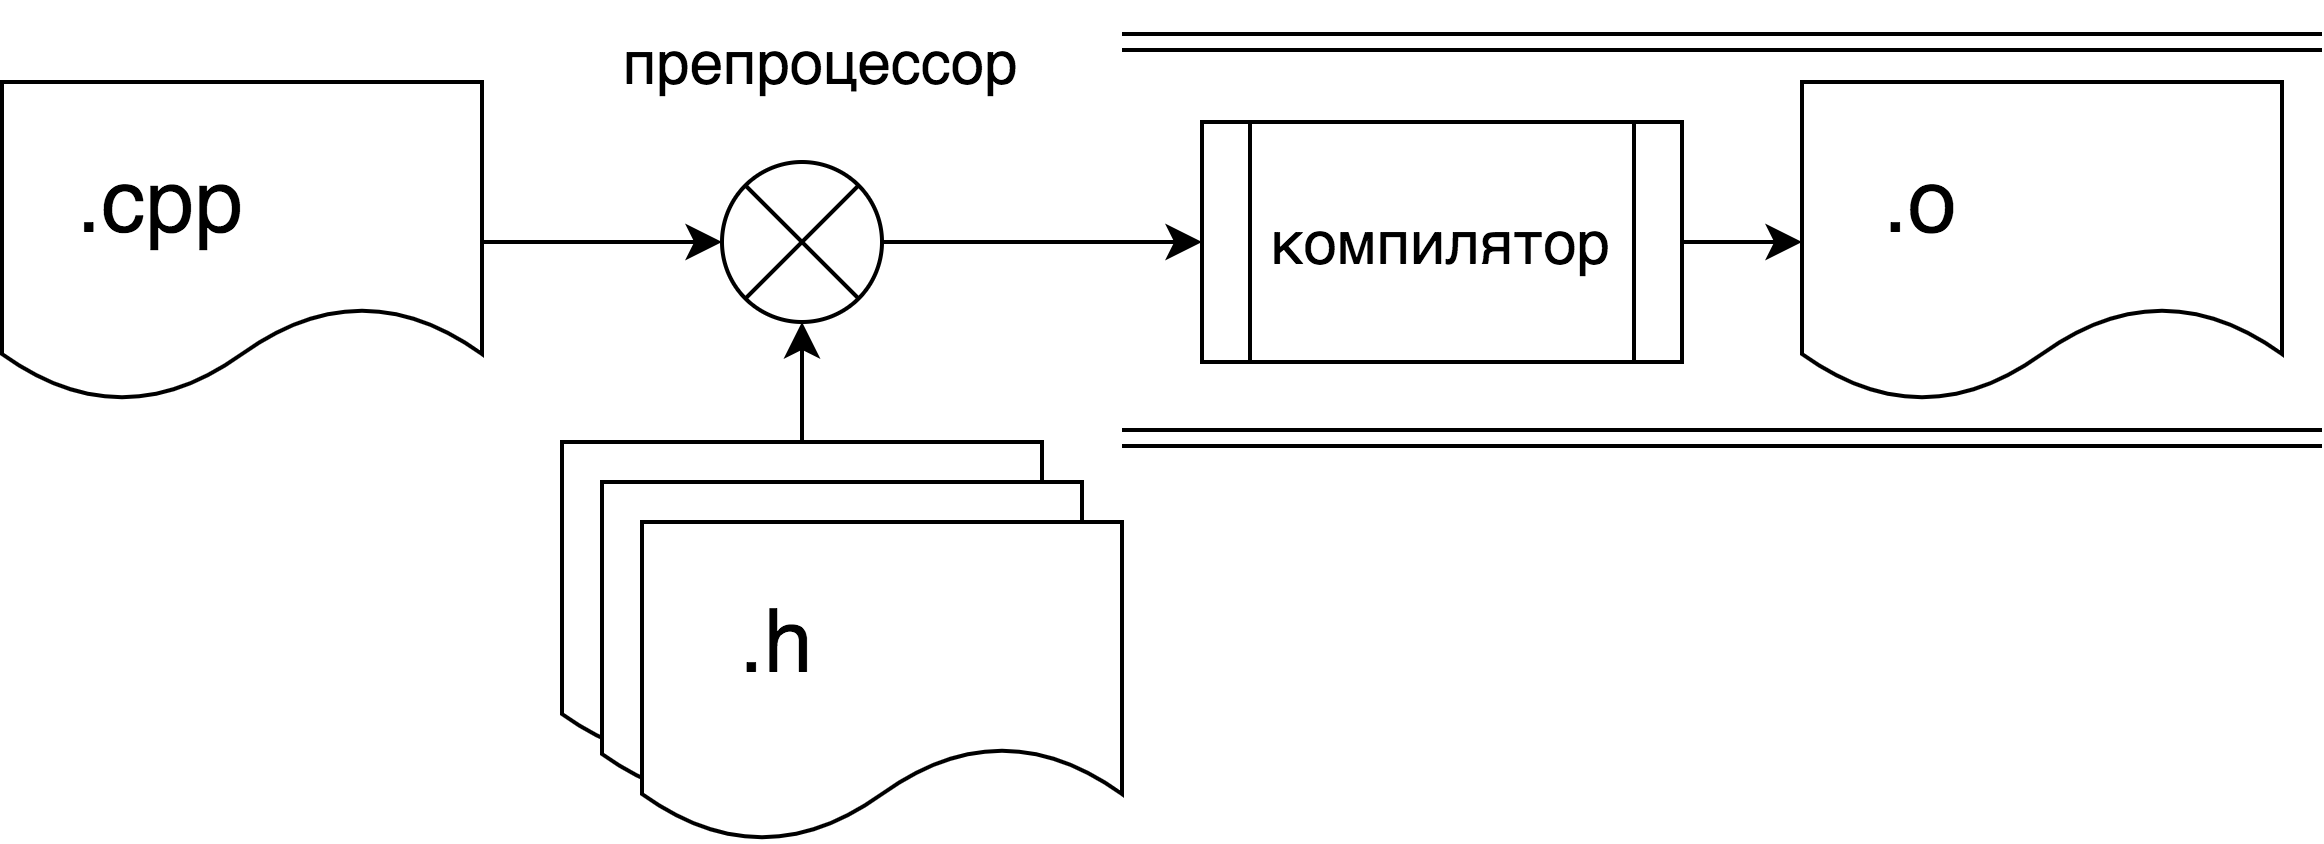
\includegraphics[align=c,width=11cm,keepaspectratio]{images/translation_unit.png}
\end{frame}

\begin{frame}[fragile]{Объявление и определение}
  \[
    \mathbf{declaration} \neq \mathbf{definition}
  \]

  \vspace{0.3em}

  \begin{itemize}
    \item объявление функций
    \item предварительное объявление классов
    \item предварительное объявление \lstinline{enum}
    \item объявление внешней (\lstinline{extern}) переменной
    \item объявление статического члена класса
    \item объявление шаблонного параметра
    \item объявление псевдонима типа
    \item \lstinline{using} объявление
    \item явное объявление инстанциации шаблона
    \item специализация шаблона без определения
  \end{itemize}
\end{frame}

\begin{frame}[fragile]{Объявления}
  \begin{lstlisting}[basicstyle=\ttfamily\srcbigsize]
    int f(double);
    class C;
    enum class E;
    extern int a;
    extern int a;

    struct S
    {
      static S s;
      //static S s;
    };

    using T = int;
    using std::cout;

    template <class T>
    int g();
    template <>
    int g<double>();

    template <class T> class X;
    template <> class X<int>;
  \end{lstlisting}
\end{frame}

\begin{frame}{Уникальность определений}
  One definition rule (\textbf{ODR})

  \vspace{2em}

  В одной единице трансляции допустимо лишь одно определение любой переменной, функции, класса, \lstinline{enum} или шаблона.

  \vspace{2em}

  Во всей программе допустимо лишь одно определение функции или переменной, которая ODR-используется (иначе -- \textbf{UB}).
\end{frame}

\begin{frame}{Повторение определений}
  Во всей программе может быть более одного определения класса, \lstinline{enum}, шаблона, если:

  \vspace{1em}

  \begin{itemize}
    \item каждый вариант определения состоит из одинаковой последовательности токенов \vspace{1em}
    \item поиск имени, связанного с каждым таким определением, во всех случаях дает ту же сущность \vspace{1em}
    \item любые связанные операторы и методы должны давать вызов одной и той же функции в каждом случае
  \end{itemize}
\end{frame}

\begin{frame}{ODR-использование}
  \begin{itemize}
    \item объект ODR-используется, если его значение читается (если только это не константа с известным на момент компиляции значением), записывается, его адрес берётся или с ним связывается ссылка \vspace{2em}
    \item функция ODR-используется, если она вызывается или её адрес берётся
  \end{itemize}
\end{frame}

\begin{frame}[fragile]{Пример ODR-использования}
  \begin{lstlisting}
    struct S
    {
      static const int x = 0; // declaration
    };

    const int S::x; // definition

    int main(int argc, char ** argv)
    {
      const int & x = S::x; // S::x is ODR-used
      return S::x; // S::x is not ODR-used
    }
  \end{lstlisting}
\end{frame}

\begin{frame}[fragile]{\lstinline{inline}}
  \begin{lstlisting}[basicstyle=\ttfamily\srcbigsize]
    inline void f()
    {
      // ...
    }

    inline int x = 0;

    struct S
    {
      bool empty()
      {
        return true;
      }

      friend bool operator == (const S & lhs, const S & rhs)
      { return true; }

      static constexpr double pi = 3.14;
    };
  \end{lstlisting}
\end{frame}

\begin{frame}{Linkage}
  Имя, обозначающее объект, ссылку, функцию, тип, шаблон, пространство имен или значение, может иметь linkage (связывание).

  \vspace{0.5em}

  \begin{itemize}
    \item отсутствие связывания: имя является локальным для своей области видимости  \vspace{0.5em}
    \item внешнее связывание: имя в разных единицах трансляции ссылается на одну и ту же сущность \vspace{0.5em}
    \item внутреннее связывание: имя в любых областях видимости данной единицы трансляции ссылается на одну и ту же сущность
  \end{itemize}
\end{frame}

\begin{frame}[fragile]{Назначение связывания по умолчанию}
  \begin{itemize}
    \item отсутствие связывания
      \begin{itemize}
        \item локальные переменные без \lstinline{extern}
        \item локальные классы
        \item иные имена, объявленные на уровне блока
      \end{itemize}
    \item внешнее связывание
      \begin{itemize}
        \item глобальные не-\lstinline{const} не-\lstinline{inline} переменные
        \item глобальные \lstinline{inline} переменные
        \item функции
        \item классы
        \item шаблоны
      \end{itemize}
    \item внутреннее связывание
      \begin{itemize}
        \item глобальные \lstinline{const} не-\lstinline{inline} переменные
        \item члены анонимных \lstinline{union}
        \item сущности, объявленные в анонимном пространстве имён
      \end{itemize}
  \end{itemize}
\end{frame}

\begin{frame}[fragile]{Явное назначение связывания}
  \begin{itemize}
    \item \lstinline{extern} -- спецификатор объявления переменных, позволяющий явно задать внешнее связывание \vspace{0.5em}
    \item \lstinline{static} -- спецификатор определения глобальных переменных или функций, явно задающий внутреннее связывание
  \end{itemize}
  \begin{lstlisting}
    extern int x; // external, declaration
    extern int y = 101; // external, definition
    int z = 111; // external
    static int u = -1; // internal
    const int v = 9; // internal
    static const int w = 3; // internal
    inline const int s = 3; // external
    extern const int t = 1; // external
  \end{lstlisting}
\end{frame}

\begin{frame}[fragile]{Language linkage}
  Имена переменных и функций с внешним связыванием обладают свойством ``language linkage''.

  \vspace{1em}

  Можно задать явно: \\

  \vspace{0.7em}

  \lstinline{extern} \emph{string-literal} \lstinline|{ ... }|

  \lstinline{extern} \emph{string-literal} \emph{declaration}

  \vspace{1em}

  где \emph{string-literal}:

  \begin{itemize}
    \item \lstinline{"C++"}
    \item \lstinline{"C"}
  \end{itemize}
\end{frame}

%-------------------------------------------------
\section{Препроцессор}

\begin{frame}[fragile]{Директивы препроцессора}
  \lstinline{#} \emph{директива [аргументы]}

  \vspace{1em}

  Директива должна размещаться на одной строке, занимает всю строку.

  \begin{itemize}
    \item \lstinline{define}
    \item \lstinline{undef}
    \item \lstinline{include}
    \item \lstinline{if}, \lstinline{ifdef}, \lstinline{ifndef}, \lstinline{else}, \lstinline{elif}, \lstinline{endif}
    \item \lstinline{error}
    \item \lstinline{pragma}
    \item \lstinline{line}
  \end{itemize}
\end{frame}

\begin{frame}[fragile]{\lstinline{pragma}}
  \lstinline{#pragma} \emph{params}

  \begin{lstlisting}
    #pragma once

    #pragma pack(1)
    struct S
    {
      char a;
      int b;
      short c;
    };
  \end{lstlisting}
\end{frame}

\begin{frame}[fragile]{\lstinline{error}}
  \lstinline{#error} \emph{message}

  \begin{lstlisting}
    #if defined(__clang__)
    // clang
    #elif defined(__GNUC__) || defined(__GNUG__)
    // gcc
    #elif defined(_MSC_VER)
    // MSVC
    #else
    #  error "Unsupported compiler"
    #endif
  \end{lstlisting}
\end{frame}

\begin{frame}[fragile]{\lstinline{line}}
  \begin{itemize}
    \item \lstinline{#line} \emph{lineno}
    \item \lstinline{#line} \emph{lineno} \lstinline{"}\emph{filename}\lstinline{"}
  \end{itemize}
  \begin{lstlisting}
    std::cout << __FILE__ << ":" << __LINE__ << std::endl;
  #line 333 "foo.def"
    std::cout << __FILE__ << ":" << __LINE__ << std::endl;
  \end{lstlisting}
\end{frame}

\begin{frame}[fragile]{Условные директивы}
  \begin{lstlisting}
    #ifdef identifier
    #ifndef identifier
    #if expression
    #elif expression
    #else
    #endif
  \end{lstlisting}
\end{frame}

\begin{frame}[fragile]{Условные директивы, конструкция}
  \begin{lstlisting}
    #ifdef / ifndef / if
    // main case
    ...
    #elif ...
    // alternative case
    ...
    #else
    // else case
    ...
    #endif
  \end{lstlisting}
\end{frame}

\begin{frame}[fragile]{Условные директивы, выражения}
  \begin{enumerate}
    \item подстановка макросов \vspace{1em}
    \item оператор \lstinline{defined id} или \lstinline{defined(id)} \rarr \lstinline{1} или \lstinline{0} \vspace{1em}
    \item оператор \lstinline{__has_include(...)} \rarr \lstinline{1} или \lstinline{0} \vspace{1em}
    \item прочие идентификаторы \rarr \lstinline{0} (кроме \lstinline{true}/\lstinline{false}) \vspace{1em}
    \item базовые токены \rarr токены \vspace{1em}
    \item вычисление выражения, как константного
  \end{enumerate}
\end{frame}

\begin{frame}[fragile]{Условные директивы, пример}
  \begin{lstlisting}
    //#define FOO
    //#define X 3 * 1 + 0
    #if !defined(FOO)
        std::cout << "First" << std::endl;
    #elif X == 3
        std::cout << "Second" << std::endl;
    #else
    #  ifndef BAR
        std::cout << "Third" << std::endl;
    #  endif
    #endif
  \end{lstlisting}
\end{frame}

\begin{frame}[fragile]{\lstinline{include}}
  \begin{itemize}
    \item \lstinline{#include <} \emph{файл} \lstinline{>} -- ``стандартные'' или ``глобальные'' файлы \vspace{1em}
    \item \lstinline{#include "} \emph{файл} \lstinline{"} -- ``локальные'' файлы
  \end{itemize}

  \vspace{2em}

  Выражение для \lstinline{__has_include} имеет такую же форму и смысл.
\end{frame}

\begin{frame}[fragile]{Заголовочные файлы}
  \textbf{a.h}:
  \begin{lstlisting}[basicstyle=\ttfamily\srcbigsize]
    int max(int a, int b);
    inline const double pi = 3.14;
  \end{lstlisting}

  \vspace{0.5em}

  \textbf{a.cpp}:
  \begin{lstlisting}[basicstyle=\ttfamily\srcbigsize]
    void f() {}
    #include "a.h"
    #include "a.h"
    int x = max(10, 100);
  \end{lstlisting}

  \vspace{0.5em}

  \textbf{a.i}:
  \begin{lstlisting}[basicstyle=\ttfamily\srcbigsize]
    void f() {}
    int max(int a, int b);
    inline const double pi = 3.14;
    int max(int a, int b);
    inline const double pi = 3.14;
    int x = max(10, 100);
  \end{lstlisting}
\end{frame}

\begin{frame}[fragile]{Защита от повторного включения}
  ``Include guards'':
  \begin{lstlisting}
    #ifndef SOME_UNIQUE_HEADER_NAME
    #define SOME_UNIQUE_HEADER_NAME

    ...
    #endif
  \end{lstlisting}

  \vspace{2em}

  Альтернатива:
  \begin{lstlisting}
    #pragma once
  \end{lstlisting}
\end{frame}

%-------------------------------------------------
\section{Макросы}

\begin{frame}[fragile]{Макросы}
  \begin{lstlisting}
    #define identifier
    #define identifier replacement
    #define identifier(parameters) replacement
    #define identifier(parameters, ...) replacement
    #define identifier(...) replacement
    #undef identifier
  \end{lstlisting}
\end{frame}

\begin{frame}[fragile]{Сложные макросы}
  \begin{lstlisting}
    #define MAX(a, b) a < b ? b : a

    if (MAX(x, y) == 0) {
      ...
    }

    ->

    if (x < y ? y : x == 0) {
      ...
    }

    ->

    if ((x < y) ? (y) : (x == 0)) {
      ...
    }
  \end{lstlisting}
\end{frame}

\begin{frame}[fragile]{Ограничения макросов}
  Рекурсия запрещена

  \begin{lstlisting}
    #define foo foo

    foo
    ->
    foo
  \end{lstlisting}

  \vspace{2em}

  Вложенные вызовы разрешены

  \begin{lstlisting}
    #define foo(x) x

    foo(foo(foo(1)))
    ->
    1
  \end{lstlisting}
\end{frame}

\begin{frame}{Особенности подстановки параметров}
  В подстановке сложных макросов параметры дополнительно раскрываются.

  \vspace{1em}

  Этапы подстановки:

  \vspace{0.5em}

  \begin{enumerate}
    \item Определение мест вхождения параметров в строке замены и их первичная подстановка \vspace{0.7em}
    \item Раскрытие параметров в местах их подстановки \vspace{0.7em}
    \item В строке замены обрабатываются макросы (при этом явно запрещена рекурсия)
  \end{enumerate}
\end{frame}

\begin{frame}[fragile]{Специальные операции подстановки}
  В подстановке сложных макросов \lstinline{#} и \lstinline{##} играют особую роль:

  \vspace{2em}

  \begin{itemize}
    \item stringification (литерация): \lstinline{#a}, где \lstinline{a} -- параметр макроса; вместо обычной подстановки параметра, параметр превращается в корректный строковый литерал (с обрамляющими \lstinline{""}) и подставляется в строку замены \vspace{1em}
    \item concatenation (склейка): \lstinline{##} между любыми двумя параметрами или между параметром и другим токеном вызывает конкатенацию результатов их подстановки (препроцессор проверит корректность полученного токена)
  \end{itemize}
\end{frame}

\begin{frame}[fragile]{Примеры stringification и concatenation}
  \begin{lstlisting}
    #define show(a, b, c) #a #b #c

    show(x, 10, "hello\n")
    ->
    "x10\"hello\\n\""


    #define print(type) void print_ ## type (type x) { ... }

    print(char)
    ->
    void print_char(char x) { ... }
  \end{lstlisting}
\end{frame}

\begin{frame}[fragile]{Особенности stringification и concatenation}
  При этом \lstinline{#} и \lstinline{##} оказывает влияние на обработку параметров макросов: литерация или склейка производятся \textbf{до} возможного раскрытия параметров.

  \vspace{1em}

  \begin{lstlisting}
    #define foo ABC
    #define concat(a) foo ## a

    concat(__LINE__)
    ->
    foo__LINE__
  \end{lstlisting}
\end{frame}

\begin{frame}[fragile]{Обход особенностей stringification и concatenation}
  Обойти раннюю обработку операций \lstinline{#} и \lstinline{##} можно двойным перенаправлением:

  \begin{lstlisting}
    #define show(x) do_show(x)
    #define do_show(x) #a

    show(__LINE__)
    ->
    "123"

    #define concat(a, b) do_concat(a, b)
    #define do_concat(a, b) a ## b

    concat(0x, __LINE__)
    ->
    0x123
  \end{lstlisting}
\end{frame}

\begin{frame}[fragile]{Защита параметров макросов}
  \begin{lstlisting}
    #define MAX(a, b) a < b ? b : a

    MAX(0, x & 0xFF)
    ->
    0 < x & 0xFF ? x & 0xFF : 0
  \end{lstlisting}

  \vspace{1em}

  \begin{lstlisting}
    #define MAX(a, b) (a) < (b) ? (b) : (a)
    MAX(0, x & 0xFF)
    ->
    (0) < (x & 0xFF) ? (x & 0xFF) : (0)
  \end{lstlisting}
\end{frame}

\begin{frame}[fragile]{Защита тела макросов}
  \begin{lstlisting}
    #define MAX(a, b) (a < b ? b : a)

    if (MAX(x, y) == 0) {
      ...
    }
    ->
    if ((x < y ? y : x) == 0) {
      ...
    }
  \end{lstlisting}
\end{frame}

\begin{frame}[fragile]{Защита места вставки}
  \begin{lstlisting}
    #define PRINT(x) do { \
      ...; \
      ...; \
    } while (false)

    // Now this is OK:
    if (...)
      PRINT(...);
    else
      ...;
  \end{lstlisting}
\end{frame}

\begin{frame}[fragile]{Побочные эффекты в макросах}
  \begin{lstlisting}
    #define MAX(a, b) (a) < (b) ? (b) : (a)

    MAX(x++, --y);
    ->
    (x++) < (--y) < (--y) : (x++);
  \end{lstlisting}
\end{frame}

\end{document}
